%<dscrpt>Fichier de déclarations Latex à inclure au début d'un élément de cours.</dscrpt>

\documentclass[a4paper]{article}
\usepackage[hmargin={1.8cm,1.8cm},vmargin={2.4cm,2.4cm},headheight=13.1pt]{geometry}

%includeheadfoot,scale=1.1,centering,hoffset=-0.5cm,
\usepackage[pdftex]{graphicx,color}
\usepackage[french]{babel}
%\selectlanguage{french}
\addto\captionsfrench{
  \def\contentsname{Plan}
}
\usepackage{fancyhdr}
\usepackage{floatflt}
\usepackage{amsmath}
\usepackage{amssymb}
\usepackage{amsthm}
\usepackage{stmaryrd}
%\usepackage{ucs}
\usepackage[utf8]{inputenc}
%\usepackage[latin1]{inputenc}
\usepackage[T1]{fontenc}


\usepackage{titletoc}
%\contentsmargin{2.55em}
\dottedcontents{section}[2.5em]{}{1.8em}{1pc}
\dottedcontents{subsection}[3.5em]{}{1.2em}{1pc}
\dottedcontents{subsubsection}[5em]{}{1em}{1pc}

\usepackage[pdftex,colorlinks={true},urlcolor={blue},pdfauthor={remy Nicolai},bookmarks={true}]{hyperref}
\usepackage{makeidx}

\usepackage{multicol}
\usepackage{multirow}
\usepackage{wrapfig}
\usepackage{array}
\usepackage{subfig}


%\usepackage{tikz}
%\usetikzlibrary{calc, shapes, backgrounds}
%pour la présentation du pseudo-code
% !!!!!!!!!!!!!!      le package n'est pas présent sur le serveur sous fedora 16 !!!!!!!!!!!!!!!!!!!!!!!!
%\usepackage[french,ruled,vlined]{algorithm2e}

%pr{\'e}sentation du compteur de niveau 2 dans les listes
\makeatletter
\renewcommand{\labelenumii}{\theenumii.}
\renewcommand{\thesection}{\Roman{section}.}
\renewcommand{\thesubsection}{\arabic{subsection}.}
\renewcommand{\thesubsubsection}{\arabic{subsubsection}.}
\makeatother


%dimension des pages, en-t{\^e}te et bas de page
%\pdfpagewidth=20cm
%\pdfpageheight=14cm
%   \setlength{\oddsidemargin}{-2cm}
%   \setlength{\voffset}{-1.5cm}
%   \setlength{\textheight}{12cm}
%   \setlength{\textwidth}{25.2cm}
   \columnsep=1cm
   \columnseprule=0.5pt

%En tete et pied de page
\pagestyle{fancy}
\lhead{MPSI-\'Eléments de cours}
\rhead{\today}
%\rhead{25/11/05}
\lfoot{\tiny{Cette création est mise à disposition selon le Contrat\\ Paternité-Pas d'utilisations commerciale-Partage des Conditions Initiales à l'Identique 2.0 France\\ disponible en ligne http://creativecommons.org/licenses/by-nc-sa/2.0/fr/
} }
\rfoot{\tiny{Rémy Nicolai \jobname}}


\newcommand{\baseurl}{http://back.maquisdoc.net/data/cours\_nicolair/}
\newcommand{\urlexo}{http://back.maquisdoc.net/data/exos_nicolair/}
\newcommand{\urlcours}{https://maquisdoc-math.fra1.digitaloceanspaces.com/}

\newcommand{\N}{\mathbb{N}}
\newcommand{\Z}{\mathbb{Z}}
\newcommand{\C}{\mathbb{C}}
\newcommand{\R}{\mathbb{R}}
\newcommand{\D}{\mathbb{D}}
\newcommand{\K}{\mathbf{K}}
\newcommand{\Q}{\mathbb{Q}}
\newcommand{\F}{\mathbf{F}}
\newcommand{\U}{\mathbb{U}}
\newcommand{\p}{\mathbb{P}}


\newcommand{\card}{\mathop{\mathrm{Card}}}
\newcommand{\Id}{\mathop{\mathrm{Id}}}
\newcommand{\Ker}{\mathop{\mathrm{Ker}}}
\newcommand{\Vect}{\mathop{\mathrm{Vect}}}
\newcommand{\cotg}{\mathop{\mathrm{cotan}}}
\newcommand{\sh}{\mathop{\mathrm{sh}}}
\newcommand{\ch}{\mathop{\mathrm{ch}}}
\newcommand{\argsh}{\mathop{\mathrm{argsh}}}
\newcommand{\argch}{\mathop{\mathrm{argch}}}
\newcommand{\tr}{\mathop{\mathrm{tr}}}
\newcommand{\rg}{\mathop{\mathrm{rg}}}
\newcommand{\rang}{\mathop{\mathrm{rg}}}
\newcommand{\Mat}{\mathop{\mathrm{Mat}}}
\newcommand{\MatB}[2]{\mathop{\mathrm{Mat}}_{\mathcal{#1}}\left( #2\right) }
\newcommand{\MatBB}[3]{\mathop{\mathrm{Mat}}_{\mathcal{#1} \mathcal{#2}}\left( #3\right) }
\renewcommand{\Re}{\mathop{\mathrm{Re}}}
\renewcommand{\Im}{\mathop{\mathrm{Im}}}
\renewcommand{\th}{\mathop{\mathrm{th}}}
\newcommand{\repere}{$(O,\overrightarrow{i},\overrightarrow{j},\overrightarrow{k})$}
\newcommand{\cov}{\mathop{\mathrm{Cov}}}

\newcommand{\absolue}[1]{\left| #1 \right|}
\newcommand{\fonc}[5]{#1 : \begin{cases}#2 \rightarrow #3 \\ #4 \mapsto #5 \end{cases}}
\newcommand{\depar}[2]{\dfrac{\partial #1}{\partial #2}}
\newcommand{\norme}[1]{\left\| #1 \right\|}
\newcommand{\se}{\geq}
\newcommand{\ie}{\leq}
\newcommand{\trans}{\mathstrut^t\!}
\newcommand{\val}{\mathop{\mathrm{val}}}
\newcommand{\grad}{\mathop{\overrightarrow{\mathrm{grad}}}}

\newtheorem*{thm}{Théorème}
\newtheorem{thmn}{Théorème}
\newtheorem*{prop}{Proposition}
\newtheorem{propn}{Proposition}
\newtheorem*{pa}{Présentation axiomatique}
\newtheorem*{propdef}{Proposition - Définition}
\newtheorem*{lem}{Lemme}
\newtheorem{lemn}{Lemme}

\theoremstyle{definition}
\newtheorem*{defi}{Définition}
\newtheorem*{nota}{Notation}
\newtheorem*{exple}{Exemple}
\newtheorem*{exples}{Exemples}


\newenvironment{demo}{\renewcommand{\proofname}{Preuve}\begin{proof}}{\end{proof}}
%\renewcommand{\proofname}{Preuve} doit etre après le begin{document} pour fonctionner

\theoremstyle{remark}
\newtheorem*{rem}{Remarque}
\newtheorem*{rems}{Remarques}

\renewcommand{\indexspace}{}
\renewenvironment{theindex}
  {\section*{Index} %\addcontentsline{toc}{section}{\protect\numberline{0.}{Index}}
   \begin{multicols}{2}
    \begin{itemize}}
  {\end{itemize} \end{multicols}}


%pour annuler les commandes beamer
\renewenvironment{frame}{}{}
\newcommand{\frametitle}[1]{}
\newcommand{\framesubtitle}[1]{}

\newcommand{\debutcours}[2]{
  \chead{#1}
  \begin{center}
     \begin{huge}\textbf{#1}\end{huge}
     \begin{Large}\begin{center}Rédaction incomplète. Version #2\end{center}\end{Large}
  \end{center}
  %\section*{Plan et Index}
  %\begin{frame}  commande beamer
  \tableofcontents
  %\end{frame}   commande beamer
  \printindex
}


\makeindex
\begin{document}
\noindent

\debutcours{Une théorie de l'intégration sur un segment}{0.7 \tiny{le \today}}

\section{Cahier des charges}
Une intégrale est un nombre associé à un objet géométrique (disons $\Omega$) et un objet analytique (disons $f$). On note
\begin{displaymath}
 \int_{\Omega}f
\end{displaymath}
Un intégrale n'est ni une fonction ni un objet géométrique du type aire. L'image que l'on doit avoir d'une intégrale est plutôt celle de la masse d'un objet pesant. On peut alors voir $\Omega$ comme l'étendue dans l'espace occupée par l'objet matériel et $f$ comme la fonction densité de masse. De nombreuses théories sont possibles dans des cadres divers. Les propriétés suivantes sont requises.
\begin{description}
 \item[Additivité par rapport aux objets géométriques]. Relation de Chasles. La masse d'une tige formée à partir de deux tiges soudées est la somme des deux masses des tiges qui la constituent.
\item[Linéarité par rapport à l'élément fonctionnel].
\item[Positivité]. Lorsque la \og densité\fg~ est positive, la masse est positive.
\item[Comportement pour des fonctions constantes]. La masse d'une tige homogène est le produit de la longueur par la densité (constante dans ce cas particulier).
\end{description}
La théorie de l'intégration au programme de la classe est construite pour les fonctions \emph{continues par morceaux} définies sur un segment et à valeur réelle. Une brève généralisation aux fonctions à valeurs complexes continues par morceaux est présentée.\newline
Les contraintes de comportement vis à vis des fonctions constantes et d'additivité conduisent à s'intéresser d'abord aux fonctions dites \emph{en escalier}

\section{Intégration des fonctions en escalier}
\subsection{Subdivisions}\index{subdivision}
\begin{defi}[Subdivision]
 Une subdivision d'un segment $[a,b]$ est une famille finie $(x_0,x_1,\cdots,x_n)$ telle que 
\begin{displaymath} 
 a=x_0 < x_1 < \cdots < x_n=b
\end{displaymath}
\end{defi}

\begin{rem}
\begin{itemize}
 \item Il faut bien faire la différence entre une subdivision $\mathcal S = (x_0,\cdots,x_n)$ et l'ensemble de ses valeurs $\{x_0,\cdots,x_n\}$.
\item Toute partie finie de $[a,b]$ contenant $a$ et $b$ est l'ensemble des valeurs d'une unique subdivision obtenue en rangeant par ordre croissant les éléments.
\index{pas de la subdivision}
\item On appelle \emph{pas de la subdivision} $\mathcal S = (x_0,\cdots,x_n)$ le nombre noté $\delta(\mathcal S)$ égal à la plus grande distance entre deux points consécutifs de la subdivision.
\begin{displaymath}
 \delta(\mathcal S) = \max \{x_{1}-x_0, x_2 -x_1,\cdots , x_n -x_{n-1}\}
\end{displaymath}
\end{itemize}
\end{rem}
\index{subdivision régulière}
\begin{defi}[Subdivision régulière]
Une subdivision $\mathcal S = (x_0,\cdots,x_n)$ de $[a,b]$ est régulière lorsque pour tout $k$ entre $0$ et $n-1$ :
\begin{displaymath}
 x_{k+1} - x_k = \dfrac{b-a}{n}
\end{displaymath}
\end{defi}

\begin{defi}
 Soit $\mathcal S = (x_0,\cdots,x_n)$ et $\mathcal S^\prime = (x^\prime_0,\cdots,x^\prime_n)$ deux subdivisions de $[a,b]$. On dira que $\mathcal S^\prime$ est plus fine que $\mathcal S$ lorsque $\{x_0,\cdots,x_n\}\subset \{x^\prime_0,\cdots,x^\prime_n\}$.
\end{defi}

\begin{propn}
 Soit $\mathcal S = (x_0,\cdots,x_n)$ et $\mathcal S^\prime = (x^\prime_0,\cdots,x^\prime_n)$ deux subdivisions de $[a,b]$. Il existe alors une subdivision $\mathcal S''$ plus fine que $\mathcal S$ et que $\mathcal S^\prime$.
\end{propn}
\begin{demo}
 Il suffit de former la subdivision constituée à partir de l'ensemble égal à l'union des ensembles associés à $\mathcal S$ et $\mathcal S^\prime$.
\end{demo}

\subsection{Fonctions en escalier}
\begin{figure}[h!]
 \centering
 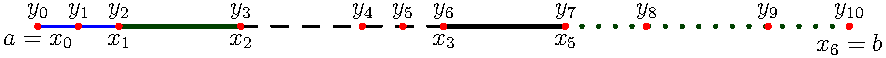
\includegraphics{C2189_1.pdf}
 % C2189_1.pdf: 0x0 pixel, 0dpi, 0.00x0.00 cm, bb=
 \caption{Subdivisions adaptées}
 \label{fig:C2189_1}
\end{figure}
\index{fonction en escalier}\index{subdivision adaptée}
\begin{defi}[Fonction en escalier- Subdivision adaptée]
 Une fonction $\varphi$ définie sur un segment $[a,b]$ est dite en escalier lorsqu'il existe une subdivision $\mathcal S = (x_0,\cdots,x_n)$ de $[a,b]$ telle que : pour chaque entier $i$ entre $0$ et $n-1$, la restriction de $\varphi$ à l'intervalle ouvert $]x_i,x_{i+1}[$ est constante.\newline
Une telle subdivision est dite adaptée à $\varphi$.\newline
L'ensemble des fonctions en escalier sur $[a,b]$ est noté $\mathcal E ([a,b])$.
\end{defi}
\begin{exples} 
Les fonctions considérées sont définies sur un intervalle $[a,b]$. \newline
Une fonction nulle sauf en un nombre fini de points est en escalier.\newline
La restriction de la fonction caractéristique de $\Q$ n'est pas en escalier. 
\end{exples}

\begin{rem}
 Une fonction en escalier admet plusieurs subdivisions adaptées. En particulier, si $\mathcal S$ est adaptée à une fonction en escalier $\varphi$ et si $\mathcal S^\prime$ est plus fine que $\mathcal S$ alors $\mathcal S^\prime$ est adaptée à $\varphi$.
\end{rem}

\begin{propn} \label{prop:escal_op}
Pour toutes fonctions $\varphi$ et $\psi$ en escalier sur $[a,b]$  et tout nombre réel $\lambda$:
\begin{align*}
 \varphi + \psi &,& \lambda \varphi &,& \varphi\psi &,& \sup(\varphi,\psi) &,& \inf(\varphi,\psi)
\end{align*}
sont  en escalier sur $[a,b]$.
\end{propn}
\begin{demo}
 Notons $\mathcal S_\varphi$ une subdivision adaptée à $\varphi$ et $\mathcal S_\psi$ une subdivision adaptée à $\psi$. Considérons alors une subdivision $\mathcal S$ plus fine que $\mathcal S_\varphi$ et $\mathcal S_\psi$. Sur un intervalle ouvert constitué par deux points consécutifs de $\mathcal S$, les restrictions \emph{des deux} fonctions sont constantes; il en est donc de même pour les restrictions des fonctions proposées par la proposition (opérations fonctionnelles).
\end{demo}
\begin{rem}
 La proposition précédente peut se reformuler de la manière suivante.
\begin{quote}
 L'ensemble $\mathcal E ([a,b])$ des fonctions en escalier sur $[a,b]$ est une sous-algèbre stable pour les opérations $\sup$ et $\inf$ de l'algèbre $\mathcal F ([a,b])$ de toutes les fonctions définies dans $[a,b]$ (à valeurs réelles).
\end{quote}
\end{rem}
\begin{propn}
 Une fonction en escalier sur $[a,b]$
\begin{itemize}
 \item prend un nombre fini de valeurs, elle est donc bornée.
 \item admet en chaque point des limites à gauche et à droite (strictement)
 \item admet un ensemble fini de points de discontinuités.
\end{itemize}
\end{propn}
\begin{demo}
 Conséquence immédiate de la définition.
\end{demo}

\subsection{Intégrale des fonctions en escalier}\index{intégrale des fonctions en escalier}
\begin{nota}
 Soit $\varphi$ une fonction en escalier et $\mathcal S=(x_0,\cdots,x_n)$ une subdivision adaptée à $\varphi$ telle que $v_i$ soit la valeur de $\varphi$ sur $]x_i,x_{i+1}[$. On note
\begin{displaymath}
 I_\mathcal{S}(\varphi)= \sum_{i=0}^{n-1}(x_{i+1}-x_i)v_i.
\end{displaymath}
\end{nota}
\begin{propn}
 Soit $\varphi$ une fonction en escalier et $\mathcal S$, $\mathcal S'$ deux subdivisions adaptées. Alors
\begin{displaymath}
 I_\mathcal{S}(\varphi)=I_{\mathcal{S}'}(\varphi).
\end{displaymath}
\end{propn}
\begin{defi}
 L'intégrale d'une fonction en escalier $\varphi$ définie sur un segment $[a,b]$ est la valeur commune de toutes les sommes $I_\mathcal{S}$ pour toutes les subdivisions adaptées $\mathcal S$. Elle est notée
\begin{displaymath}
 \int_{[a,b]}\varphi.
\end{displaymath}
\end{defi}
\begin{rems}
 \begin{itemize}
  \item L'intégrale d'une fonction en escalier nulle sauf en un nombre fini de points est nulle.
  \item La définition de l'intégrale des fonctions en escalier traduit exactement la dernière des propriétés requises au début. La masse d'une tige de densité constante est le produit de cette densité par la longueur de la tige. Dans la sous-section suivante, on vérifie les autres propriétés du cahier des charges.
 \end{itemize}
\end{rems}

\subsection{Validation du cahier des charges}
 \subsubsection{Additivité}
 \begin{propn}\label{prop:chasles0}
  Soit $[a,b]$ un segment ($a<b$), $c \in ]a,b[$ et $\varphi$ une fonction définie dans $[a,b])$. Alors $\varphi$ est en escalier sur $[a,b]$ si et seulement si ses restrictions aux segments $[a,c]$ et $[c,b]$ sont en escalier.  On a alors:
  \[
   \int_{[a,c]}\varphi_{|[a,c]} + \int_{[c,b]}\varphi_{|[c,b]} = \int_{[a,c]}\varphi.
  \]
 \end{propn}
\begin{rem}
 En général, on ne note pas le marqueur de restriction et on écrit simplement
  \[
   \int_{[a,c]}\varphi + \int_{[c,b]}\varphi = \int_{[a,c]}\varphi.
  \]
\end{rem}

\begin{demo}
 Supposons $\varphi \in \mathcal{E}([a,b])$ et considérons une subdivision de $[a,b]$ adaptée à $\varphi$. On ajoute le point $c$ à cette subdivision s'il n'y est pas et on la partitionne en des subdivisions de $[a,c]$ et $[c,b]$. Ces subdivisions sont alors adaptées aux restrictions.\newline
 Réciproquement, si les deux restrictions sont en escalier, o
en concatènant deux subdivisions adaptées aux restrictions, on forme une subdivision adaptée à $\varphi$. La formule pour les intégrales est immédiate avec la définition par une somme.
\end{demo}
La notation la plus simple et la plus générale d'une intégrale place l'élément géométrique en bas. Introduisons une nouvelle notation, un peu plus compliquée mais commode.
\begin{nota}\index{notation du domaine d'intégration}
 Soit $\varphi \in \mathcal{E}([a,b])$. On définit les notations $\int_{a}^{b}f$ et $\int_{b}^{a}f$ par :
\[
 \int_{a}^{b}f = \int_{[a,b]}f , \hspace{1cm} \int_{b}^{a}f = -\int_{[a,b]}f,\hspace{1cm}\text{on convient aussi que } \int_{a}^{a}f = 0.
\]
\end{nota}
\begin{propn}\label{prop:chasles}
 Soit $I$ un segment de $\R$, $\varphi \in \mathcal{E}(I)$ et $u$, $v$, $w$ dans $I$. Les restrictions de $\varphi$ sont en escalier et
\[
 \int_u^v \varphi + \int_v^w\varphi = \int_u^w \varphi.
\]
\end{propn}
\begin{demo}
 La démonstration consiste à vérifier la formule avec la proposition \ref{prop:chasles0} en considérant tous les rangements possibles pour $u$, $v$, $w$.
\begin{center}
\renewcommand{\arraystretch}{1.2}
\begin{tabular}{|l|c|c|c|c|c|c|} \hline
Cas           & 1                 & 2                 & 3                 & 4                 & 5                 & 6 \\ \hline
Configuration & $u \leq v \leq w$ & $u \leq w \leq v$ & $v \leq u \leq w$ & $v \leq w \leq u$ & $w \leq v \leq u$ & $w \leq u \leq v$ \\ \hline
\end{tabular}
\end{center}
Le cas 1 est la traduction directe de la proposition \ref{prop:chasles0}.\newline
Examinons le cas 4 (les autres se traitent de la même manière). On applique la proposition \ref{prop:chasles0} aux intervalles $[v,w]$ et $[w,u]$:
\[
\int_{[v,w]}\varphi +  \int_{[w,u]}\varphi = \int_{[v,u]}\varphi 
\Rightarrow
\int_{v}^{w}\varphi - \int_{u}^{w}\varphi = -\int_{u}^{v}\varphi
\Rightarrow 
\int_{u}^{v}\varphi + \int_{v}^{w}\varphi = \int_{u}^{w}\varphi.
\]
\end{demo}

\subsubsection{Linéarité}
\begin{propn}
Soit $\varphi$ et $\psi$ dans $\mathcal{E}([a,b])$, $\lambda\in \R$. 
\[
 \int_{[a,b]}\left( \varphi + \psi\right) = \int_{[a,b]} \varphi + \int_{[a,b]} \psi, \hspace{1cm} \int_{[a,b]}\lambda \varphi = \lambda \int_{[a,b]}\varphi.
\]
\end{propn}
\begin{demo}
 Immédiat avec la définition de l'intégrale d'une fonction en escalier et une subdivision assez fine pour être adaptée aux deux fonctions.
\end{demo}
\begin{rem}
 On a vu que l'intégrale d'une fonction nulle sauf en un nombre fini de points était nulle. Par linéarité, si deux fonctions en escalier sont égales sauf sur un nombre fini de points, elles ont la même intégrale.
\end{rem}
 
\subsubsection{Positivité}
\begin{propn}
 Soit $\varphi \in \mathcal{E}([a,b])$. Si $\varphi \geq 0$ (c'est à dire $\forall x \in[a,b], \varphi(x) \geq 0$) alors $\int_{[a,b]}\varphi \geq 0$.
\end{propn}
\begin{demo}
 Immédiat avec la définition de l'intégrale.
\end{demo}
\begin{propn}
 Soit $\varphi$ et $\psi$ dans $\mathcal{E}([a,b])$.
\[
 \varphi \leq \psi \Rightarrow \int_{[a,b]}\varphi \leq \int_{[a,b]}\psi, \hspace{1cm} \left|\int_{[a,b]}\varphi \right| \leq \int_{[a,b]}|\varphi|.
\]
\end{propn}
\begin{demo}
 Signalons d'abord que la valeur absolue d'une fonction en escalier est une fonction en escalier (prop \ref{prop:escal_op}).\newline
 La première inégalité est une conséquence de la linéarité et de la positivité appliquées à l'intégrale de $\psi - \varphi\geq 0$. La seconde propriété résulte de la première appliquée à $-|\varphi| \leq \varphi \leq |\varphi|$.  
\end{demo}


\section{Intégrales inférieure et supérieure d'une fonction bornée}
Considérons une fonction $f$ définie sur un segment $[a,b]$ et \emph{bornée}. Par exemple, il existe $M>0$ tel que :
\begin{displaymath}
 \forall x\in [a,b] : -M\leq f(x) \leq M
\end{displaymath}
On définit alors deux ensembles notés $\mathcal E_-(f)$ et $\mathcal E_+(f)$ formés respectivement par les fonctions en escalier qui minorent et qui majorent $f$. Si $\varphi$ est une fonction en escalier:
\begin{align*}
 \varphi \in \mathcal E_-(f) &\Leftrightarrow \forall x\in [a,b] : \varphi(x) \leq f(x) \\
 \varphi \in \mathcal E_+(f) &\Leftrightarrow \forall x\in [a,b] :  f(x) \leq \varphi(x)
\end{align*}
Ces ensembles sont non vides car la fonction constante égale à $-M$ est dans $\mathcal E_-(f)$ et la fonction constante égale à $M$ est dans $\mathcal E_+(f)$. Il est à noter que
\begin{displaymath}
 \forall \varphi\in \mathcal E_- , \forall \psi\in \mathcal E_+, \forall x\in[a,b] :
\varphi(x) \leq f(x) \leq \psi(x)
\end{displaymath}
Introduisons maintenant les parties $\mathcal I_-(f)$ et $\mathcal I_+(f)$ de $\R$ définies par :
\begin{align*}
 \mathcal I_-(f) = \left\lbrace \int_{[a,b]}\varphi , \; \varphi \in \mathcal E_-(f)\right\rbrace  & &
 \mathcal I_+(f) = \left\lbrace \int_{[a,b]}\varphi , \; \varphi \in \mathcal E_+(f)\right\rbrace
\end{align*}
Ces parties se majorent et minorent mutuellement :
\begin{propn}
\begin{displaymath}
 \forall I\in \mathcal I_-(f), \forall J\in \mathcal I_+(f) : I\leq J
\end{displaymath}
\end{propn}
\begin{demo}
 En effet, il existe des fonctions en escalier $\varphi\in\mathcal E_-(f)$ et  $\psi\in\mathcal E_-(f)$ telles que 
\begin{align*}
 I= \int_{[a,b]}\varphi & & J= \int_{[a,b]}\psi
\end{align*}
De plus 
\begin{multline*}
 \forall x\in[a,b] : \varphi(x) \leq f(x) \leq \psi(x) \Rightarrow \forall x\in[a,b] : \psi(x)-\varphi(x)\geq 0 
\Rightarrow J-I = \int_{[a,b]}(\psi -\varphi)\geq 0
\end{multline*}
par linéarité et positivité.
\end{demo}
On peut donc définir les \emph{intégrales inférieure et supérieure} notées $I_-(f)$ et $I_+(f)$ par :
\begin{align*}
 I_-(f) = \sup( \mathcal I_-(f))   & & I_+(f) = \inf(  \mathcal I_+(f) )
\end{align*}
On peut décréter d'appeler \emph{intégrables} les fonctions bornées pour lequelles les intégrales inférieures et supérieures sont égales. Cela conduit à une théorie de l'intégration (parmi bien d'autres) qui n'est pas celle au programme de la classe.\newline
En MPSI, on convient de n'appeler \og intégrables\fg~ que les \emph{fonctions continues par morceaux}. L'objet des prochaines sections est de montrer que pour une fonction \emph{continue par morceaux} les intégrales supérieures et inférieures sont égales et que \og l'intégrale des fonctions continues par morceaux sur un segment\fg~ainsi définie vérifie le cahier des charges.

\section{Fonctions uniformément continues}
\begin{defi}
 Une fonction $f$ définie sur un intervalle $I$ est dite \emph{uniformément continue} si et seulement si :
\begin{displaymath}
 \forall \varepsilon>0, \exists \alpha_\varepsilon \text{ tel que : }\forall (x,y)\in I^2, |x-y|<\alpha \Rightarrow |f(x)-f(y)|<\varepsilon.
\end{displaymath}
\end{defi}
\index{continuité uniforme}
\begin{rem}
 Toute fonction $k$-lipschitzienne est uniformément continue.
\end{rem}

\index{théorème de Heine}
\begin{thm}[Théorème de Heine] \label{prop:Heine}
 Toute fonction continue sur un segment est uniformément continue.
\end{thm}
\begin{demo}
On va montrer l'implication contraposée.\newline
Soit $f$ définie sur un segment $I=[a,b]$ qui \emph{ n'est pas uniformément continue}. Il existe alors un $\varepsilon >0$ tel que, pour tout $\alpha>0$, il existe $x$ et $y$ dans $I$ tels que $|x-y|\leq \alpha$ et $|f(x)-f(y)|\geq \varepsilon$.\newline
\`A cause du $\forall \alpha$, on peut considérer des $\alpha$ de la forme $\frac{1}{n}$ pour $n\in\N^*$. Marquons bien la dépendance des $x$ et $y$ vis à vis de ce $\alpha=\frac{1}{n}$. L proposition se traduit par l'existence de deux suites $(x_n)_{n\in\N^*}$ et $(y_n)_{n\in\N^*}$ telles que :
\begin{displaymath}
 \forall n\in \N^* : |x_n -y_n|\leq \frac{1}{n} \text{ et } |f(x_n)-f(y_n)|\geq \varepsilon.
\end{displaymath}
Comme $I$ est un segment, la suite $(x_n)_{n\in\N^*}$ est bornée. D'après le théorème de Bolzano-Weirstrass\index{théorème de Bolzano Weirstrass}, on peut extraire une suite convergente, c'est à dire qu'il existe une partie infinie $\mathcal I$ de $\N^*$ telle que $(x_n)_{n\in\mathcal I}$ converge. On note $x$ sa limite.\newline
Le théorème d'encadrement et la relation $|x_n -y_n|\leq \frac{1}{n}$ montrent que la suite $(y_n)_{n\in\mathcal I}$ converge aussi vers $x$. On peut alors utiliser la continuité de $f$ en $x$ pour former une contradiction par passage à la limite à partir de
\begin{displaymath}
 \forall n\in \mathcal J :  |f(x_n)-f(y_n)|\geq \varepsilon
\end{displaymath}
car les deux suites $(f(x_n))_{n\in\mathcal J}$ et $(f(y_n))_{n\in\mathcal J}$ convergent vers $f(x)$.
\end{demo}
\begin{rem}
 Exemple de fonction continue mais non uniformément sur un intervalle. Soit $f$ une fonction uniformément continue sur un intervalle $I$. On peut montrer en \href{http://back.maquisdoc.net/v-1/index.php?act=chelt&id_elt=4798}{exercice} qu'il existe des réels $a$ et $b$ tels que $f(x)\leq a+b|x|$ pour tous les $x\in I$. On en déduit qu'une fonction uniformément continue sur un intervalle borné est bornée. Une fonction continue mais non bornée sur un intervalle borné n'est donc pas uniformément continue.
\end{rem}

\section{Intégration des fonctions continues par morceaux}
\begin{figure}[h!t]
 \centering
 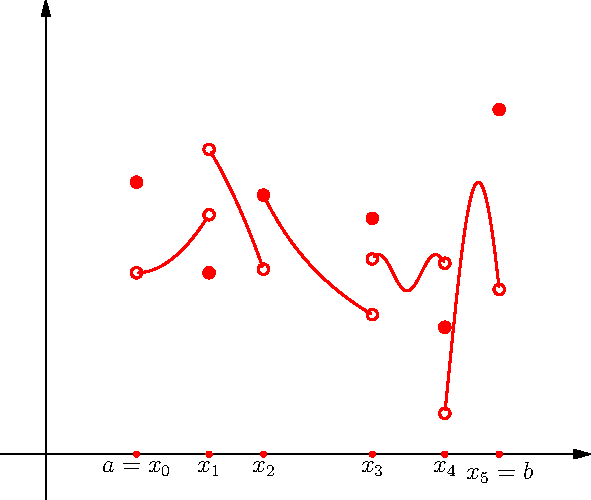
\includegraphics[width=10cm]{C2189_2.pdf}
 % C2189_2.pdf: 0x0 pixel, 0dpi, nanxnan cm, bb=
 \caption{Fonction continue par morceaux}
 \label{fig:C2189_2}
\end{figure}

\subsection{Fonctions continues par morceaux}\index{fonction continue par morceaux}
La notion suivante n'est pas au programme mais permet de bien comprendre la situation.\index{fonction réglée}
\begin{defi}[fonction réglée]
 Une fonction $f$ définie sur un segment $\left[a, b \right]$ est dite \emph{réglée} si et seulement si $f$ admet une limite strictement à droite en tout $x\in \left[ a, b \right[$, et elle admet une limite strictement à gauche en tout $x\in ]a,b]$. 
\end{defi}
Une fonction $f$ réglée sur $\left[a,b\right]$ est continue en $x\in \left]a , b \right[$ si et seulement si
\[
 \lim_{x^{--}} = f(x) = \lim_{x^{++}}.
\]
\begin{exple}
  Les fonctions en escalier sont continues par morceaux. Les restrictions aux intervalles ouverts attachés à une subdivision adaptée sont constantes.
\end{exple}

\begin{defi}
 Une fonction $f$ définie sur un segment $[a,b]$ est dite en continue par morceaux lorsqu'il existe une subdivision $\mathcal S = (x_0,\cdots,x_n)$ de $[a,b]$ telle que : pour chaque entier $i$ entre $0$ et $n-1$, la restriction de $f$ à l'intervalle ouvert $]x_i,x_{i+1}[$ est continue et prolongeable par continuité au segment $[x_i,x_{i+1}]$.\newline
Une telle subdivision est dite adaptée à $f$.\newline
L'ensemble des fonctions continues par morceaux sur $[a,b]$ est noté $\mathcal C_{pm} ([a,b])$.
\end{defi}

\begin{nota}
 Dans les conditions de la définition, on convient de noter $f_i$ le prolongement continu à $\left[ x_i,x_{i+1}\right] $ de la restriction de $f$ à $\left] x_i,x_{i+1}\right[ $. Comme $f_i$ est une fonction \emph{continue sur un segment}, elle est bornée et atteint ses bornes. On note donc
\begin{align*}
 M_i = \max_{[x_i,x_{i+1}]}f_i &,& m_i = \min_{[x_i,x_{i+1}]}f_i
\end{align*}
\end{nota}

\begin{rem}
  La condition de prolongeabilité par continuité signifie que la fonction admet une limite finie strictement à droite de $x_0, x_1, \cdots ,x_{n-1}$ et une limite finie strictement à gauche de $x_1, x_2, \cdots x_n$. On peut utiliser cette remarque pour caractériser les fonctions continues par morceaux.
\end{rem}
\begin{rem}
 Si $f$ n'est pas continue en $x$, on dit que $x$ est un point de discontinuité de $f$. Une fonction continue par morceaux est une fonction réglée avec un nombre fini de points de discontinuités.
\end{rem}


\begin{propn}
\begin{itemize}
\item Une fonction continue par morceaux est bornée.
\item Une fonction continue par morceaux est continue en chaque point du segment sauf peut-être aux points de la subvision. Aux points de la subdivision elle admet  des limites finies à gauche (sauf en $a$) et à droite (sauf en $b$) strictement.
 \item Pour toutes fonctions $f$ et $g$ continues par morceaux sur $[a,b]$  et tout nombre réel $\lambda$:
\begin{align*}
 f + g &,& \lambda f &,& f g &,& \sup(f, g) &,& \inf(f,g)
\end{align*}
sont  continues par morceaux sur $[a,b]$.
\end{itemize}
\end{propn}
\begin{demo}
 \begin{itemize}
 \item Avec les notations précisées plus haut :
\begin{displaymath}
 \forall x\in[a,b], \hspace{0.5cm} f(x) 
\left\lbrace  
\begin{aligned}
  \geq& \min \{m_0,m_1,\cdots ,m_{n-1},f(x_0),f(x_1),\cdots ,f(x_n)\} \\
  \leq& \max \{M_0,M_1,\cdots ,M_{n-1},f(x_0),f(x_1),\cdots ,f(x_n)\}
\end{aligned}
\right. 
\end{displaymath}
\item Si $u$ n'est pas un point de la subdivision, il est dans un intervalle ouvert sur lequel la restriction de $f$ est continue. La fonction $f$ est donc continue en $u$. La fonction admet des limites finies strictement de chaque côté d'un point de la subdivision à cause de la condition de prolongement.
\item Les stabilités pour les opérations se vérifient comme pour les fonctions en escalier en considérant une subdivision assez fine pour être adaptée à toutes les fonctions. En se plaçant dans un intervalle ouvert défini par des points consécutifs de cette subdivision, on peut utliser les résultats relatifs aux opérations sur les fonctions convergentes.
\end{itemize}
\end{demo}
\begin{figure}[h!t]
 \centering
 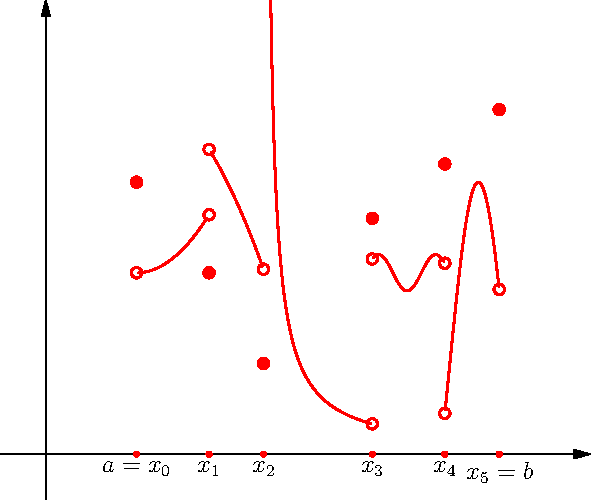
\includegraphics[width=10cm]{C2189_3.pdf}
 \caption{Une fonction qui \emph{n'est pas} continue par morceaux}
 \label{fig:C2189_3}
\end{figure}

\begin{propn}
 Toute fonction continue par morceaux est la somme d'une fonction continue et d'une fonction en escalier. Avec les notations de l'algèbre linéaire:
\begin{displaymath}
  \mathcal{C}_{pm}([a,b]) = \mathcal{C}([a,b]) + \mathcal{E}([a,b]).
\end{displaymath}
\end{propn}
L'ensemble des fonctions continues par morceaux est donc le plus petit espace vectoriel contenant les deux classes de fonctions élémentaires intéressantes. On peut remarquer que la somme n'est pas directe car l'intersection est formée par les fonctions constantes. 
\begin{demo}
 L'inclusion $\mathcal{C}([a,b]) + \mathcal{E}([a,b])\subset \mathcal{C}_{pm}([a,b])$ est évidente car les fonctions continues comme les fonctions en escalier sont continues par morceaux. Prouvons l'inclusion réciproque.\newline
 Toute fonction $f$ continue par morceaux est réglée, c'est à dire qu'elle admet partout des limites strictement à gauche et à droite. Introduisons des fonctions \og sauts \fg~ à gauche et à droite
 \[
  s_{-,f}(x) = 
\left\lbrace 
\begin{aligned}
 &0& &\text{ si } x = a\\
 &f(x) - \left(\lim_{\substack{t \rightarrow x \\ t < x}}f(t)\right)& &\text{ si } x \in \left] a, b\right]
\end{aligned}
\right. 
, \hspace{1cm}
  s_{+,f}(x) = 
\left\lbrace 
\begin{aligned}
 &\left(\lim_{\substack{t \rightarrow x \\ t > x}}f(t)\right) - f(x)& &\text{ si } x \in \left[ a,b \right[\\
 0 &\text{ si } x = b
\end{aligned}
\right. 
 \]
\`A cause des résultats sur la convergence des fonctions, l'opération qui à une fonction associe un saut est linéaire:
\[
  \forall (f,g) \in \mathcal{C}_{pm}([a,b]), \forall \lambda \in \R, \; 
  \left\lbrace
  \begin{aligned}
    s_{-, f+g} &= s_{-,f} + s_{-,g} \\s_{-,\lambda f} &= \lambda s_{-,f}
  \end{aligned}
  \right. , \hspace{0.5cm}
  \left\lbrace
  \begin{aligned}
    s_{+, f+g} &= s_{+,f} + s_{+,g} \\s_{+,\lambda f} &= \lambda s_{+,f}
  \end{aligned}
  \right. . 
\]
Les sauts de $f$ sont des fonctions nulles sauf aux points où $f$ est discontinue. 
Introduisons des fonctions qui somment les sauts de $f$
\[
 \forall x \in [a,b],\; S_-(x) = \sum_{t \leq x} s_{-,f}(t)
 ,\hspace{0.5cm}
 S_+(x) = \sum_{t < x} s_{+,f}(t) \text{ avec } S_{+}(0) = 0.
\]
Ces fonctions sont bien définies car une fonction continue par morceaux n'admet qu'un nombre fini de discontinuités donc seul un nombre fini de $t$ contribuent vraiment à chaque somme. De plus, elles sont en escalier et reproduisent les sauts de $f$:
\[
  s_{-,S_-} = s_{-,f},\; s_{+,S_-} = 0, \hspace{0.5cm} s_{-,S_+} = 0,\; s_{+,S_+} = s_{+,f}.
\]
Notons $S = S_- + S_+$ et $g = f - s$. Par linéarité les sauts de $g$ à gauche et à droite sont nuls donc elle est continue. On a obtenu la décomposition
\[
 f = \underset{\text{en escalier}}{\underbrace{S}} + \underset{\text{continue}}{\underbrace{g}}.
\]
\end{demo}

\subsection{Approximations}
\index{théorème d'approximation des fonctions continues par morceaux}
\begin{thm}[Approximation des fonctions continues par morceaux]
 Soit $f$ une fonction continue par morceaux sur $[a,b]$. Pour tout $\varepsilon>0$, il existe des fonctions en escalier $\varphi$ et $\psi$ telles que pour tout $x\in[a,b]$ :
\begin{align*}
 \varphi(x) \leq f(x) \leq \psi(x) &,& \psi(x) - \varphi(x)\leq \varepsilon
\end{align*}
\end{thm}
\begin{demo}
 Ce théorème est admis. Sa démonstration repose sur l'utilisation du théorème de Heine appliqué aux fonctions $f_i$.
\end{demo}

\begin{exple}
 Les fonctions (dites de Darboux) sont des fonctions en escalier qui encadrent une fonction $f$ continue. par morceaux  Elles sont définies de la manière suivante.\newline
 Soit $\mathcal S =(x_0,x_1,\cdots x_n)$ une subdivision adaptée à $f$. Pour $i$ entre $0$ et $n-1$, on note $f_i$ le prolongement continu à $[x_i,x_{i+1}]$ de la restriction de $f$ à $]x_i,x_{i+1}[$. Chaque fonction $f_i$ est continue sur son segment de définition, elle est donc bornée et atteint ses bornes notées $m_i$ et $M_i$.\newline
On définit $\forall x\in[a,b]$ les fonctions de Darboux inférieure ($\varphi_-$) et supérieure ($\varphi_+$) par : 
\begin{align*}
\varphi_{-}(x) &= 
\begin{cases}
f(x_i) \text{ si } \exists i \text{ tel que } x=x_i\\
m_i \text{ si } \exists i \text{ tel que } x\in ]x_i,x_{i+1}[
\end{cases}\\
\varphi_{+}(x) &= 
\begin{cases}
f(x_i) \text{ si } \exists i \text{ tel que } x=x_i\\
M_i \text{ si } \exists i \text{ tel que } x\in ]x_i,x_{i+1}[
\end{cases}
\end{align*}
On a alors $\varphi_{-}(x)\leq f(x) \leq \varphi_{+}(x)$ pour tous les $x$ de $[a,b]$. Ces fonctions peuvent être utilisées pour démontrer le théorème d'approximation en considérant des subdivisions assez fines dont le pas est donné par le théorème de Heine.
\end{exple}

\subsection{Définition}
\index{intégrale des fonctions continues par morceaux}
\begin{propn}
Pour une fonction continue par morceaux, l'intégrale inférieure est égale à l'intégrale supérieure. 
\end{propn}
\begin{demo}
 Soit $f$ une fonction continue par morceaux sur $[a,b]$. D'après le théorème d'approximation, pour tout $\varepsilon >0$, il existe deux fonctions en escalier $\varphi\in \mathcal E_-(f)$ et $\psi\in \mathcal E_+(f)$ telles que
\begin{displaymath}
 \forall x \in [a,b] : 
 0 \leq \psi(x) - \varphi(x) \leq \varepsilon
\end{displaymath}
Par linéarité et positivité,
\begin{displaymath}
 \int_{[a,b]}\psi - \int_{[a,b]}\varphi = \int_{[a,b]}(\psi - \varphi) \leq \int_{[a,b]}\varepsilon = (b-a)\varepsilon
\end{displaymath}
Par définition des intégrales inférieure et supérieure et d'après l'encadrement précédent,
\begin{displaymath}
 \int_{[a,b]}\varphi \leq I_-(f) \leq I_+(f) \int_{[a,b]}\psi \Rightarrow
0 \leq I_+(f) - \leq I_-(f) \leq \int_{[a,b]}\psi - \int_{[a,b]}\varphi \leq (b-a)\varepsilon
\end{displaymath}
Mais comme $b-a$ et fixé et $\varepsilon$ arbitraire,
\begin{displaymath}
I_+(f) \leq I_-(f) \Rightarrow  I_+(f) = I_-(f)
\end{displaymath}
\end{demo}
\begin{defi}
Pour une fonction continue par morceaux $f$ sur un segment $[a,b]$, la valeur commune de l'intégrale inférieure et de l'intégrale supérieure est appelée l'intégrale de $f$ et notée
\begin{displaymath}
 \int_{[a,b]}f
\end{displaymath}
\end{defi}

\section{Propriétés - Validation du cahier des charges}
\index{intégrale : additivité - relation de Chasles}
Les démonstrations proposées sont toutes du même type. Elle comprennent des majorations et se terminent par un raisonnement à la Cauchy.
\subsection{Additivité - Relation de Chasles}
\index{intégrale : linéarité}
\begin{propn}
 Soit $a$, $b$, $c$ trois réels tels que $a<b<c$ et $f$ une fonction quelconque définie dans $[a,c]$. 
\begin{displaymath}
 f\in\mathcal{C}_{pm}([a,c])\Leftrightarrow
 f_{|[a,b]}\in\mathcal{C}_{pm}([a,b]) \text{ et } f_{|[b,c]}\in\mathcal{C}_{pm}([b,c])
\end{displaymath}
Dans ce cas on a
\begin{displaymath}
 \int_{[a,c]}f = \int_{[a,b]}f + \int_{[b,c]}f
\end{displaymath}
\end{propn}
\begin{demo}
 La première équivalence se démontre facilement en introduisant le point $b$ dans les subdivisions de $[a,c]$.\newline
Pour l'égalité des intégrales, considérons un $\varepsilon>0$ quelconque. D'après le théorème d'approximation, il existe des fonctions en escalier $\varphi_\varepsilon$ et $\psi_\varepsilon$ qui encadrent $f$ et telles que $\psi_\varepsilon -\varphi_\varepsilon \leq \varepsilon$ sur $[a,c]$ donc aussi sur $[a,b]$ et $[b,c]$. On peut donc écrire
\begin{align*}
 \int_{[a,c]}\varphi_\varepsilon \leq \int_{[a,c]}f \leq \int_{[a,c]}\psi_\varepsilon  & &\times +1 \\ 
 \int_{[a,b]}\varphi_\varepsilon \leq \int_{[a,b]}f \leq \int_{[a,b]}\psi_\varepsilon  & & \times -1\\
 \int_{[b,c]}\varphi_\varepsilon \leq \int_{[b,c]}f \leq \int_{[b,c]}\psi_\varepsilon  & & \times -1
\end{align*}
En soustrayant les deux dernières à la première, on obtient
\begin{displaymath}
 \int_{[a,c]}\varphi_\varepsilon - \int_{[a,b]}\psi_\varepsilon - \int_{[b,c]}\psi_\varepsilon
\leq \int_{[a,c]}f -\int_{[a,b]}f - \int_{[b,c]}f \leq
 \int_{[a,c]}\psi_\varepsilon - \int_{[a,b]}\varphi_\varepsilon - \int_{[b,c]}\varphi_\varepsilon 
\end{displaymath}
En utilisant les propriétés de l'intégrale des fonctions en escalier (additivité, linéarité), on obtient
\begin{displaymath}
 \left| \int_{[a,c]}f -\int_{[a,b]}f - \int_{[b,c]}f \right|
\leq \int_{[a,c]}\left(\psi_\varepsilon - \varphi_\varepsilon \right) 
\leq (b-a)\varepsilon
\end{displaymath}
Comme $\varepsilon$ est un réel strictement positif quelconque, cela entraine l'égalité.
\end{demo}

\begin{nota}
 Comme pour les fonctions en escalier, on introduit de nouvelles notations. Soit $f$ une fonction continue par morceaux sur un intervalle $[a,b]$ avec $a<b$. 
\[
 \int_{a}^bf = \int_{[a,b]}f, \hspace{0.5cm}\int_{b}^af =  - \int_{[a,b]}f =-\int_{a}^bf, \hspace{0.5cm}\text{on convient aussi que } \int_{a}^af =0.
\]
\end{nota}
Avec ces notations, on peut reformuler la proposition précedente sous la forme d'une\index{relation de Chasles} relation de Chasles
\begin{propn}[relation de Chasles] \label{prop: chaslesCPM}
 Soit $f$ une fonction continue par morceaux dans $[a,b]$ et soit $c\in[a,b]$. Soit $u$, $v$, $w$ trois réels deux à deux distincts parmi $a$, $b$, $c$. Alors:
\begin{displaymath}
 \int_{u}^vf + \int_{v}^wf = \int_{u}^wf 
\end{displaymath}
\end{propn}
\begin{demo}
 La démonstration est analogue à celle de la proposition \ref{prop:chasles}. On considére toutes les configurations possibles des lettres et on se ramène dans chaque cas à la proposition formulée avec des intégrales sur des segments.
\end{demo}

\subsection{Linéarité}
\begin{propn}
 Soient $f$ et $g$ deux fonctions continues par morceaux sur un segment $[a,b]$ et $\lambda \in \R$.
\begin{displaymath}
 \int_{[a,b]}\left( f+g\right) = \int_{[a,b]} f + \int_{[a,b]}g, \hspace{1cm}
 \int_{[a,b]}\lambda f = \lambda \int_{[a,b]} f
\end{displaymath}
\end{propn}
\begin{demo}
Comme la démonstration n'est pas plus simple si on se limite aux fonctions en escalier, on se place dans le cadre plus général de fonctions bornées avec des intégrales supérieures et inférieures égales.\newline
On suppose donc $f$ et $g$ bornées et telles que $I_-(f) = I_+(g)$, $I_-(f) = I_+(g)$. Il est alors clair que $f+g$ est bornée.\newline 
Le cas de la somme est traité en détail. La démarche est analogue pour le produit par $\lambda$ (en faisant attention au signe de $\lambda$).\newline
Soit $\varphi_1$ quelconque dans $\mathcal E_-(f)$ et $\varphi_2$ quelconque dans $\mathcal E_-(g)$ alors $\varphi_1 + \varphi_2 \in \mathcal E_-(f+g)$. On en déduit, par linéarité de l'intégration des fonctions en escalier et définition de $I_-$,
\begin{displaymath}
 \forall \varphi_1 \in \mathcal E_-(f), \forall \varphi_2 \in \mathcal E_-(g) :
\int_{[a,b]}\varphi_1 + \int_{[a,b]}\varphi_2 \leq I_-\left( f+g\right) . 
\end{displaymath} 
On joue avec les quantificateurs et les inégalités pour exploiter le fait que $I_-(f)$ et  $I_-(g)$ sont définies comme des bornes supérieures.
\begin{multline*}
 \forall \varphi_1 \in \mathcal E_-(f),\;\left( \forall \varphi_2 \in \mathcal E_-(g) ,\;
\int_{[a,b]}\varphi_2 \leq I_-\left( f+g\right) - \int_{[a,b]}\varphi_1 \right)  \\ 
\Rightarrow \forall \varphi_1 \in \mathcal E_-(f),\;  I_-(g) \leq I_-\left( f+g\right) - \int_{[a,b]}\varphi_1 
\Rightarrow \forall \varphi_1 \in \mathcal E_-(f),\; \int_{[a,b]}\varphi_1 \leq I_-\left( f+g\right) - I_-(g) \\
\Rightarrow I_-(f) \leq I_-\left( f+g\right) - I_-(g) 
\Rightarrow I_-(f) + I_-(g) \leq I_-\left( f+g\right) .
\end{multline*}
On procède de manière analogue avec des fonctions en escalier $\psi_1$ et $\psi_2$ au dessus de $f$ et $g$. La somme $\psi_1+\psi_2$ est dans $\mathcal E_+(f+g)$. On exploite le fait que $I_+(f+g)$, $I_+(f)$, $I_+(g)$ sont définies comme des bornes inférieures.
\begin{multline*}
 \forall \psi_1 \in \mathcal E_+(f), \forall \psi_2 \in \mathcal E_+(g) ,\; I_+\left( f+g\right) \leq \int_{[a,b]}\psi_1+\int_{[a,b]}\psi_2 \\ 
\Rightarrow \forall \psi_1 \in \mathcal E_-(f),\; \left(\forall \psi_2 \in \mathcal E_+(g),\;  I_+\left( f+g\right) - \int_{[a,b]}\psi_1\leq \int_{[a,b]}\psi_2\right) \\
\Rightarrow \forall \psi_1 \in \mathcal E_-(f),\;  I_+\left( f+g\right) - \int_{[a,b]}\psi_1\leq I_+(g) 
\Rightarrow \forall \psi_1 \in \mathcal E_-(f),\;  I_+\left( f+g\right) - I_+(g)\leq \int_{[a,b]}\psi_1 \\
\Rightarrow I_+\left( f+g\right) - I_+(g)\leq I_+(f) 
\Rightarrow I_+\left( f+g\right) \leq I_+(f) + I_+(g).
\end{multline*}
Le fait que les intégrales supérieures et inférieures de $f$ et $g$ sont égales permet de conclure
\[
 \left. 
 \begin{aligned}
  I_-(f) + I_-(g) \leq I_-\left( f+g\right) \leq I_+\left( f+g\right) \leq I_+(f) + I_+(g)\\
  I_-(f) = I_+(f) \; \text{ et } \;  I_-(g) = I_+(g)
 \end{aligned}
\right\rbrace \Rightarrow
I_-\left( f+g\right) = I_+\left( f+g\right).
\]
D'où $\int_{[a,b]}\left( f + g\right) = \int_{[a,b]}f + \int_{[a,b]}g$.
\end{demo}
\index{invariance par translation}
\begin{propn}[Invariance par translation]
Soit $f$ continue par morceaux sur un segment $[a,b]$, soit $T\in \R$. On définit la fonction $f_T$ dans $[a-T,b-T]$ par : $f_T(x)=f(T+x)$. Elle est continue par morceaux dans $[a-T,b-T]$ et vérifie
\begin{displaymath}
 \int_{a-T}^{b-T}f_T = \int_a^bf
\end{displaymath} 
\end{propn}
\begin{demo}
 Utilisons la notation de la proposition pour définir une bijection (translation) entre les ensembles de fonctions en escalier
\[
 \left\lbrace 
 \begin{aligned}
  \mathcal{E}([a-T,b-T]) &\rightarrow \mathcal{E}([a,b]) \\
  \varphi &\mapsto \varphi_T
 \end{aligned}
\right. 
\]
Elle transporte $\mathcal{E}_-(f_T)$ sur $\mathcal{E}_-(f)$ et $\mathcal{E}_+(f_T)$ sur $\mathcal{E}_+(f)$ et conserve l'intégrale d'une fonction en escalier: 
\[
 \int_{[a-T,b-T]}\varphi_T = \int_{[a,b]}\varphi .
\]  
\end{demo}
On en déduit l'égalité des intégrales pour une fonction en escalier.
\begin{rem}
 Ce résultat peut apparaitre comme une conséquence du théorème de changement de variable mais il ne suppose que $f$ soit $\mathcal{C}^1$.  
\end{rem}

\index{intégrale : positivité}
\subsection{Positivité et conséquences}
\begin{propn}[positivité de l'intégrale]
 Si $f$ est une fonction continues par morceaux sur $[a,b]$ et à valeurs positives ou nulles, alors son intégrale sur $[a,b]$ est positive ou nulle.
\end{propn}
\begin{demo}
 Comme $f$ est à valeurs positives ou nulles, la fonction $\varphi_0$ constante nulle est en escalier et dans $\mathcal{E}^-(f)$. Son intégrale est nulle. On a alors par définition de l'intégrale d'une fonction en escalier: $0\leq I_(f)=\int_{[a,b]}f$.
\end{demo}
\begin{rem}
 Si on utilise la notation intégrale avec des bornes $a$ en bas et $b$ en haut, pour utiliser la positivité, il faut faire attention à ce que les bornes soient dans le bon sens ($a\leq b$).
\end{rem}

On en déduit par linéarité les propriétés suivantes.
\begin{propn}
 Soit $f$ et $g$ continues par morceaux sur $[a,b]$ :
\begin{displaymath}
 f\leq g \Rightarrow \int_{[a,b]}f \leq \int_{[a,b]}g\text{ et } \left\vert\int_{[a,b]}f\right\vert\leq \int_{[a,b]}|f|
\end{displaymath}
\end{propn}
\begin{demo}
 Linéarité et positivité comme pour l'intégrale des fonctions en escalier.
\end{demo}

\begin{propn}
 Soit $f$ une fonction continue sur $[a,b]$ et à valeurs positives alors la nullité de l'intégrale de $f$ sur $[a,b]$ entraine que la fonction est constante de valeur $0$.
\end{propn}
\begin{figure}[h!t]
 \centering
 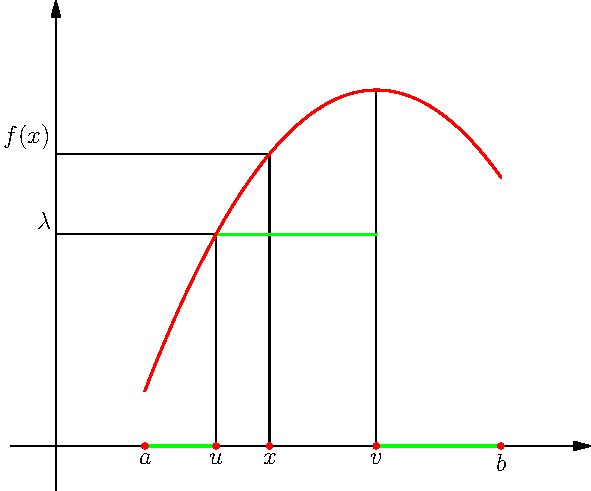
\includegraphics[width=10cm]{C2189_4.pdf}
 \caption{Intégrale d'une fonction continue à valeurs positives}
 \label{fig:C2189_4}
\end{figure}

\begin{demo}
 Supposons $f$ continue, positive et non identiquement nulle et montrons que son intégrale est strictement positive.\newline
En effet, il existe un $x$ tel que $f(x)>0$. Soit $\lambda$ un réel tel que $0<\lambda<f(x)$. Comme $f$ est continue en $x$, il existe des réels $u$ et $v$ tel que $[u,v]\subset[a,b]$ et que $f(t)\geq \lambda$ pour $t\in [u,v]$ (figure \ref{fig:C2189_4}). On peut alors minorer par additivité et positivité
\begin{displaymath}
 \int_{a}^bf \geq \int_u^vf\geq \int_u^v\lambda = (v-u)\lambda >0
\end{displaymath}
\end{demo}
\begin{propn}
 Soit $f$ une fonction continue non nulle sur $[a,b]$ dont l'intégrale est nulle. Il existe un $c$ tel que $a<c<b$ et que $f$ s'annule en $c$ en changeant de signe.
\end{propn}
\begin{demo}
 C'est une conséquence immédiate de la proposition précédente.
\end{demo}

\index{inégalité de la moyenne}
\begin{propn}[inégalité de la moyenne]
 Soient $f$ et $g$ deux fonctions continues par morceaux sur $[a,b]$ et $m$, $M$ deux nombres réels. On suppose de plus que $g$ est à valeurs positives ou nulles et que $m\leq f(x)\leq M$ pour tous les $x$ de $[a,b]$. Alors :
\begin{displaymath}
 m\int_{[a,b]}g \leq \int_{[a,b]}fg \leq M\int_{[a,b]}g
\end{displaymath}
\end{propn}
\begin{demo}
 Cela résulte de la propriété de positivité appliquée à $mg(x)\leq f(x)g(x) \leq Mg(x)$. Cet encadrement est valable car $g$ est à valeurs positives.
\end{demo}
\begin{rem}
 Ce résultat est souvent utilisé simplement avec $g$ constante de valeur $1$. Il est à rapprocher du plus simple des encadrements vu en début d'année.
\end{rem}
 \index{valeur moyenne d'une fonction}
\begin{defi}[valeur moyenne d'une fonction]
 La valeur moyenne d'une fonction $f\in \mathcal{C}_{pm}([a,b])$ est $\frac{1}{(b-a)}\int_{[a,b,)}f$.
\end{defi}
\begin{rem}
 D'après l'inégalité de la moyenne, la valeur moyenne de $f$ est comprise entre $\inf_{[a,b]}f$ et $\sup_{[a,b]}f$. Si de plus $f$ est continue, d'après le théorème de la valeur intermédaire, il existe un $c\in[a,b]$ tel que
\begin{displaymath}
 \frac{1}{(b-a)}\int_{[a,b,)}f
\end{displaymath}
\end{rem}
\index{inégalité de Cauchy-Schwarz}
\begin{propn}[inégalité de Cauchy-Schwarz]
 Soit $f$ et $g$ continues par morceaux sur $[a,b]$, alors
\begin{displaymath}
 \left\vert \int_{[a,b]}fg \right\vert \leq
\sqrt{\int_{[a,b]}f^2}\,\sqrt{\int_{[a,b]}g^2}
\end{displaymath}
De plus si $f$ et $g$ sont des fonctions continues qui vérifient l'égalité alors il existe un réel $\lambda$ tel que $g=\lambda f$.
\end{propn}
\begin{demo}
 Comme pour toutes les formules de ce type, la démonstration repose sur le fait que
\begin{displaymath}
 \lambda \rightarrow \int_{[a,b]}(f+\lambda g)^2 
\end{displaymath}
est un polynomiale du second degré et à valeurs toujours positives ou nulles. L'inégalité est équivalente à la négativité du discriminant. Lorsque le discriminant est nul, il existe un $\lambda$ annulant l'expression ce qui n'est possible que si $f+\lambda g$ est identiquement nulle lorsque les deux fonctions sont continues.
\end{demo}

\subsection{Sommes de Riemann}
\index{sommes de Riemann}
\begin{defi}
 Soit $f\in \mathcal{C}_{pm}([a,b])$ et $\mathcal{S}=(x_0,x_1,\cdots,x_n)$ une subdivision adaptée de $[a,b]$. Une \emph{somme de Riemann} attachée à $f$ et $\mathcal{S}$ est une expression de la forme
\begin{displaymath}
 \sum_{k=0}^{n-1}(x_{k+1}-x_k)V_k \text{ avec } V_k\in f_k([x_k,x_{k+1}])
\end{displaymath}
où $f_k$ est le prolongement continu de $f_{\left|]x_k,x_{k+1}[\right. }$ à $[x_k,x_{k+1}]$.
\end{defi}
\begin{exples}
 Les expressions suivantes sont des sommes de Riemann
\begin{align*}
 &\sum_{k=0}^{n-1}(x_{k+1}-x_k)f(x_k) & & &\sum_{k=0}^{n-1}(x_{k+1}-x_k)f(x_{k+1})
 & & &\sum_{k=0}^{n-1}(x_{k+1}-x_k)f(\frac{x_k + x_{k+1}}{2}) \\
 &\sum_{k=0}^{n-1}(x_{k+1}-x_k)\frac{f(x_{k})+f(x_{k+1})}{2}
 & & &\sum_{k=0}^{n-1}(x_{k+1}-x_k)\max_{[x_k,x_{k+1}]}f & & &\sum_{k=0}^{n-1}(x_{k+1}-x_k)\min_{[x_k,x_{k+1}]}f
\end{align*}
Lorsque la subdivision est régulière, $x_k = a + k\,\frac{b-a}{n}$, le pas est constant et se met en facteur. Les sommes de Riemann prennent la forme
\begin{displaymath}
 \frac{b-a}{n}\sum_{k=0}^{n-1}V_k
\end{displaymath}
En général, $V_k = f(x_k)$ ou $V_k = f(x_{k+1}$ mais on trouve des exercices pour lesquels d'autres valeurs interviennent.
\end{exples}
\begin{propn}
 Soit $f\in \mathcal{C}_{pm}([a,b])$ et $\left(R_n\right) _{n\in \N}$ une suite telle que chaque $R_n$ soit une somme de Riemann attachée à $f$ et à la subdivision régulière à $n+1$ points de $[a,b]$. Alors 
\begin{displaymath}
 \left(R_n\right) _{n\in \N} \rightarrow \int_{[a,b]}f
\end{displaymath}
\end{propn}
\begin{demo}
 Cette propriété est admise dans le cas continue par morceaux, une \href{\baseurl/C2190.pdf}{démonstration} est donnée dans le cas des fonctions $\mathcal{C}^1$.
\end{demo}

\subsection{Intégrale et aire}
Introduction axiomatique à la notion d'aire (à compléter). On peut interpréter l'intégrale d'une fonction en escalier à valeurs positives comme l'aire de la portion de plan comprise entre le graphe et l'axe des $x$. La similarité entre les propriétés de l'aire et de l'intégrale permet d'étendre cette interprétation au cas de la surface comprise entre l'axe des $x$ et le graphe d'une fonction positive et continue par morceaux.

\section{Extension aux fonctions à valeurs complexes}
\begin{defi}
Une fonction à valeurs complexes $f$ définie sur un segment $[a,b]$ est dite \emph{en escalier} si et seulement si il existe une subdivision (dite adaptée) $\mathcal S= (x_0,\cdots,c_n)$ telle que
\begin{displaymath}
 \forall i\in\{0\cdots,n-1\}: f_{|]a_i,a_{i+1}[} \text{ est constante}
\end{displaymath}
On note $\mathcal E([a,b],\C)$ l'ensemble des fonctions en escalier à valeurs complexes définies sur $[a,b]$.
\end{defi}
\begin{propn}
 Une fonction à valeurs complexes est en escalier si et seulement si les fonctions partie réelle et partie imaginaire sont en escalier.
\end{propn}
\begin{propn}
$\mathcal E([a,b],\C)$ est une $\C$-algèbre.
\end{propn}
\begin{defi}
 Une fonction à valeurs complexes $f$ définie sur un segment $[a,b]$ est dite \emph{continue par morceaux} si et seulement si les fonctions partie réelle $\Re f$ et partie imaginaire $\Im f$ sont continues par morceaux. On note $\mathcal C_{pm}([a,b],\C)$ l'ensemble des fonctions continues par morceaux. On dit alors qu'une fonction $f$ fonction est intégrable et on note
\begin{displaymath}
 \int_{[a,b]}f =  \int_{[a,b]}\Re f + i \int_{[a,b]}\Im f .
\end{displaymath}
\end{defi}
On vérifie sans difficulté que cette intégrale est additive par rapport à l'intervalle et $\C$-linéaire. La positivité mérite plus d'explications car il n'y a pas de relation d'ordre compatible avec les opérations dans $\C$. Ce qui remplace la positivité est la proposition suivante
\begin{propn}
 Si $f\in \mathcal C_{pm}([a,b],\C)$ alors $|f|\in \mathcal C_{pm}([a,b],\R)$ et
\begin{displaymath}
 \left \vert \int_{[a,b]}f \right \vert \leq \int_{[a,b]}|f|. 
\end{displaymath}
\end{propn}
\begin{demo}
 Attention, cette proposition ne se démontre pas par linéarité à partir de la définition. Il est indispensable de revenir aux fonctions en escalier.\newline
Remarquons d'abord que l'inégalité est vraie si $f$ est en escalier. Il existe une subdivision telle que 
\begin{displaymath}
 \left\vert \int_{[a,b]}f\right\vert = \left\vert\sum_{k=0}^{n-1}(x_{k+1}-x_k)v_k\right\vert \leq
\sum_{k=0}^{n-1}|x_{k+1}-x_k||v_k| = \int_{[a,b]}|f|
\end{displaymath}
Il s'agit seulement de l'inégalité triangulaire pour une somme finie de nombres complexes.\newline
Dans le cas où $f$ est continue par morceaux, notons $a$ et $b$ les fonctions parties réelle et imaginaire de $f$.\newline
Pour tout $\varepsilon>0$, d'après le théorème d'approximation, il existe des fonctions en escalier $\varphi_\epsilon$ et $\psi_\epsilon$ telles que, en notant  $\Phi_\varepsilon=\varphi_\epsilon+i\phi_\epsilon$ (fonction en escalier à valeurs complexes) 
\begin{displaymath}
\left. 
\begin{aligned}
|a-\varphi_\epsilon| \leq& \varepsilon \\ |b-\psi_\epsilon| \leq& \varepsilon  
\end{aligned}
\right\rbrace 
\Rightarrow \left|\Phi_\varepsilon - f\right| \leq \sqrt{2}\, \varepsilon .
\end{displaymath}
On en déduit
\begin{multline*}
\left| \int_{[a,b]}f \right| = \left| \int_{[a,b]}(a-\varphi_\varepsilon) + i \int_{[a,b]}(b-\psi_\varepsilon) + \int_{[a,b]}\Phi_\varepsilon\right| \hspace{0.5cm}(\text{ linéarité })\\
\leq 2(b-a)\varepsilon +  \left|\int_{[a,b]}\Phi_\varepsilon\right| \text{(inégalité triangulaire puis positivité intégrale réelle)}\\
\leq 2(b-a)\varepsilon + \int_{[a,b]}\left|\Phi_\varepsilon\right| \hspace{0.5cm} \text{(inégalité valable pour les fonctions en escalier)} \\
\leq 2(b-a)\varepsilon + \int_{[a,b]}\left|\Phi_\varepsilon - f\right|+ \int_{[a,b]}\left|f\right| \hspace{0.5cm} \text{(inégalité triangulaire puis linéarité)} \\
\leq (2+\sqrt{2})(b-a)\varepsilon + \int_{[a,b]}\left|f\right| \hspace{0.5cm} \text{(positivité)}.
\end{multline*}
On conclut avec un argument à la Cauchy ($\varepsilon$ est arbitraire).
\end{demo}
\end{document}
